\documentclass[11pt]{article}

% Change "review" to "final" to generate the final (sometimes called camera-ready) version.
% Change to "preprint" to generate a non-anonymous version with page numbers.
\usepackage[review]{acl}

% Standard package includes
\usepackage{times}
\usepackage{latexsym}

% For proper rendering and hyphenation of words containing Latin characters (including in bib files)
\usepackage[T1]{fontenc}
% For Vietnamese characters
% \usepackage[T5]{fontenc}
% See https://www.latex-project.org/help/documentation/encguide.pdf for other character sets

% This assumes your files are encoded as UTF8
\usepackage[utf8]{inputenc}

% This is not strictly necessary, and may be commented out,
% but it will improve the layout of the manuscript,
% and will typically save some space.
\usepackage{microtype}

% This is also not strictly necessary, and may be commented out.
% However, it will improve the aesthetics of text in
% the typewriter font.
\usepackage{inconsolata}

%Including images in your LaTeX document requires adding
%additional package(s)
\usepackage{graphicx}
\usepackage{amsmath,amssymb}
\usepackage{booktabs}
% Figures live in ../figures (relative to this file); also try figures/ for root-relative builds
\graphicspath{{../figures/}{figures/}}

% Hebrew words inline. cjhebrew works with pdfLaTeX, XeLaTeX and LuaLaTeX and handles
% right-to-left direction itself. Input is transliterated, e.g. \<bnyyn> = bet-nun-yod-yod-nun.
\usepackage{cjhebrew}

% If the title and author information does not fit in the area allocated, uncomment the following
%
%\setlength\titlebox{<dim>}
%
% and set <dim> to something 5cm or larger.

\title{MorphEvalHeb: Morphology-Aware Factual Consistency Evaluation\\for Hebrew Summarization}

% Author information can be set in various styles:
% For several authors from the same institution:
% \author{Author 1 \and ... \and Author n \\
%         Address line \\ ... \\ Address line}
% if the names do not fit well on one line use
%         Author 1 \\ {\bf Author 2} \\ ... \\ {\bf Author n} \\
% For authors from different institutions:
% \author{Author 1 \\ Address line \\  ... \\ Address line
%         \And  ... \And
%         Author n \\ Address line \\ ... \\ Address line}
% To start a separate ``row'' of authors use \AND, as in
% \author{Author 1 \\ Address line \\  ... \\ Address line
%         \AND
%         Author 2 \\ Address line \\ ... \\ Address line \And
%         Author 3 \\ Address line \\ ... \\ Address line}


\author{
Amit Avraham \quad Eyal Mazuz \quad Bracha Shapira \quad Lior Rokach \\
Ben-Gurion University of the Negev, Israel \\
\texttt{\{avramit,mazuze\}@post.bgu.ac.il}, \texttt{bshapira@bgu.ac.il}, \texttt{liorrk@post.bgu.ac.il}
}

%\author{
%  \textbf{First Author\textsuperscript{1}},
%  \textbf{Second Author\textsuperscript{1,2}},
%  \textbf{Third T. Author\textsuperscript{1}},
%  \textbf{Fourth Author\textsuperscript{1}},
%\\
%  \textbf{Fifth Author\textsuperscript{1,2}},
%  \textbf{Sixth Author\textsuperscript{1}},
%  \textbf{Seventh Author\textsuperscript{1}},
%  \textbf{Eighth Author \textsuperscript{1,2,3,4}},
%\\
%  \textbf{Ninth Author\textsuperscript{1}},
%  \textbf{Tenth Author\textsuperscript{1}},
%  \textbf{Eleventh E. Author\textsuperscript{1,2,3,4,5}},
%  \textbf{Twelfth Author\textsuperscript{1}},
%\\
%  \textbf{Thirteenth Author\textsuperscript{3}},
%  \textbf{Fourteenth F. Author\textsuperscript{2,4}},
%  \textbf{Fifteenth Author\textsuperscript{1}},
%  \textbf{Sixteenth Author\textsuperscript{1}},
%\\
%  \textbf{Seventeenth S. Author\textsuperscript{4,5}},
%  \textbf{Eighteenth Author\textsuperscript{3,4}},
%  \textbf{Nineteenth N. Author\textsuperscript{2,5}},
%  \textbf{Twentieth Author\textsuperscript{1}}
%\\
%\\
%  \textsuperscript{1}Affiliation 1,
%  \textsuperscript{2}Affiliation 2,
%  \textsuperscript{3}Affiliation 3,
%  \textsuperscript{4}Affiliation 4,
%  \textsuperscript{5}Affiliation 5
%\\
%  \small{
%    \textbf{Correspondence:} \href{mailto:email@domain}{email@domain}
%  }
%}

\begin{document}
\maketitle
\begin{abstract}
Automatic text summarization is one of the most challenging NLP tasks to evaluate: a good summary must jointly satisfy faithfulness, content coverage, conciseness, and fluency, and LLMs are known to struggle in low-resource languages where evaluation benchmarks are scarce.
Factuality evaluation is especially complex for morphologically rich languages such as Hebrew, where a single substitution, such as a \textit{binyan} shift, gender-agreement violation, or construct-state corruption, can reverse agency or alter factual content while remaining nearly identical at the surface level.
Standard metrics (ROUGE, BLEU, BERTScore) exhibit lower human-correlation for such languages, NLI- and QA-based pipelines (SummaC, QAFactEval) rely on English-centric models that degrade under Hebrew morphology, and translation-based adaptation introduces artifacts that obscure authentic error patterns.
We present \textbf{MorphEvalHeb}, a Hebrew-native automatic metric for scoring the factual correctness of Hebrew summaries generated by LLMs against their source article, rather than against a human reference summary. It combines a taxonomy of 26 Hebrew factual-error families derived from real LLM outputs, a morphology-aware pipeline that injects these errors into faithful summaries to create labeled contrastive data, and NeoDictaBERT classifiers trained on that data, enabling more reliable factuality assessment for morphologically rich, low-resource languages.
\end{abstract}
\section{Introduction}

Automatic text summarization is a central task in natural language processing, yet it remains among the most difficult to evaluate automatically. 
Unlike classification or translation, where reference outputs are relatively well-defined, a good summary must simultaneously satisfy multiple criteria: faithfulness to the source document, coverage of salient content, conciseness, and fluency. 
No single automated metric captures all these dimensions reliably.
Among these criteria, factual consistency is both the most consequential and the hardest to automate: human evaluations find that the majority of outputs from strong abstractive summarizers contain content unsupported by the source \citep{maynez-etal-2020-faithfulness}, and overlap-based metrics such as ROUGE correlate only weakly with human judgments of factual correctness \citep{kryscinski-etal-2019-neural}, since the most fluent, most abstractive outputs are often exactly the ones most prone to factual errors \citep{falke-etal-2019-ranking}.
This challenge is amplified in low-resource languages, where large language models (LLMs) trained predominantly on English data exhibit degraded generation quality, while the lack of native-language evaluation benchmarks makes failures difficult to detect or quantify.
Moreover, most existing summarization benchmarks and evaluation metrics primarily focus on short abstractive summaries rather than long, information-dense summaries grounded in long source documents, where factual consistency becomes substantially more difficult to maintain and evaluate.
These failures are not confined to single-shot summarization: autonomous LLM agents routinely summarize retrieved documents or tool outputs as an intermediate step before acting, so a single unfaithful summary can propagate uncorrected through every subsequent decision \citep{lin2025agenthallucination}, which makes a reliable, automatic factuality metric infrastructure for agentic use as much as for standalone summarization.

Factuality evaluation, which verifies that a generated summary does not introduce information inconsistent with the source, is particularly challenging for morphologically rich languages such as Hebrew.
Modern Hebrew combines derivational, inflectional, and concatenative morphology: tri-consonantal roots are realized through verbal and nominal templates (\textit{binyanim} and \textit{mishkalim}), agreement features encode gender, number, and person, and syntactic particles such as conjunctions, prepositions, and articles are attached directly as prefixes, while possessive and pronominal markers appear as suffixes. Consequently, whitespace-delimited tokens often fail to align with semantic units, making surface-level comparison fundamentally unreliable.

Critically, small morphological substitutions can alter factual meaning while remaining nearly identical orthographically. A \textit{binyan} shift may reverse agency, a gender-agreement violation may alter the acting entity, and a construct-state (\textit{smichut}) corruption may change possessive or attributive relations. Although some of these factual inconsistencies also appear cross-linguistically, Hebrew morphology makes generated summaries substantially more vulnerable to such errors, and in many cases the underlying cause originates directly from Hebrew-specific morphological structure. These error types frequently evade standard similarity-based metrics such as ROUGE, BLEU, ChrF, and BERTScore, which are not morphology-aware and exhibit substantially lower human correlation for morphologically rich languages.

We illustrate this with a representative example from our corpus. The source sentence reads \emph{``they will need creative solutions, because the Tourism Ministry is struggling''}, while the generated summary reads \emph{``they will need creative solutions so that the Tourism Ministry struggles''}. Replacing ``because'' with ``so that'' reverses the causal relation between the clauses while leaving most surface tokens unchanged. Despite the complete semantic inversion, similarity metrics remain high (ROUGE-1 F1 $\approx$ 0.94, BERTScore F1 $\approx$ 0.96), illustrating how Hebrew-specific connective morphology can produce factual errors that remain invisible to existing metrics.
% CHECK (audit E): on the sentence pair itself, repo code gives ROUGE-1 F1 0.53 and BERTScore 0.81 (heBERT) / 0.82 (AlephBERT),
% not 0.94 / 0.96. State which texts and settings the reported numbers used, or replace them.

Such errors are common in practice. We applied an LLM-based error finder (Gemini) to 293 Hebrew news summaries generated by five LLMs. It detected at least one factual error in 86\% of the summaries, and rated 73\% of the 408 detected errors as severe (4 or 5 on a five-point scale; Figure~\ref{fig:llm_detected_errors}).
% CHECK: confirm the Gemini model version used for the error_finder runs (code now
% defaults to gemini-2.5-pro; the finder currently calls Claude). Ideally a Hebrew
% speaker verifies a sample (~30) of the detected errors and we report agreement.

\begin{figure}[t]
\centering
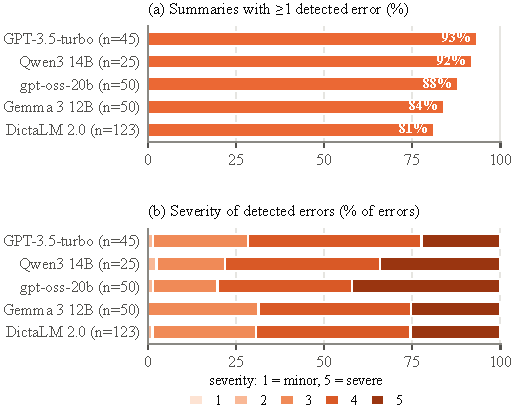
\includegraphics[width=\columnwidth]{fig_llm_detected_errors.pdf}
\caption{Factual errors detected in real Hebrew news summaries generated by five LLMs. (a) Share of summaries in which an LLM error finder (Gemini) detected at least one factual error. (b) Severity of the detected errors on the finder's 1--5 scale (5 = critical corruption of core facts, such as identity confusion or role reversal). $n$ is the number of summaries examined, pooled over detection runs. Errors were detected automatically and were not verified by human annotators.}
\label{fig:llm_detected_errors}
% CHECK (audit, provenance): about 27% (68/254) of the summaries the error finder analyzed are identical to the
% MAFAT reference (summaries_* files store the reference in `summary`; LLM outputs are in metadata.generative_summaries).
% Recompute Figure 1 on LLM outputs only before submission.
\end{figure}

Existing factuality evaluation pipelines face additional language-specific limitations. NLI-based approaches such as SummaC rely on English-only entailment models that are not trained to capture Hebrew morphological contradictions. QA-based methods such as QAFactEval depend on extractive span boundaries that become ambiguous under Hebrew morphology. Translation-based adaptation further introduces artifacts that obscure authentic Hebrew error patterns and erase distinctions that lack direct English equivalents. As a result, practitioners evaluating Hebrew LLM outputs currently lack reliable Hebrew-native factuality metrics.

We address this gap with \textbf{MorphEvalHeb}, a Hebrew-native framework that scores the factual correctness of a Hebrew summary generated by an LLM directly against its source article, with three contributions:
(1) a \textbf{Hebrew correctness-error taxonomy} of 26 fine-grained error families, derived from errors observed in real LLM-generated summaries and dominated by morpho-syntactic phenomena such as \textit{binyan}, agreement, and construct-state errors (\S\ref{sec:taxonomy});
(2) a \textbf{morphology-aware augmentation pipeline} that decomposes faithful Hebrew summaries into claims and injects controlled errors from 20 of these families, through few-shot LLM rewriting, NER-based entity swaps, and rule-based number edits, yielding labeled contrastive data (\S\ref{sec:augmentation});
and (3) \textbf{MorphEvalHeb classifiers}: a binary faithfulness verifier and a multi-label error detector fine-tuned from NeoDictaBERT, benchmarked against existing metrics and LLM judges on Hebrew summarization (\S\ref{sec:model}, \S\ref{sec:meta_eval}).

Our work is motivated by four central gaps in Hebrew LLM evaluation: limited language coverage in existing metrics, lack of morphology-aware evaluation design, scarcity of long-form correctness-oriented Hebrew benchmarks, and high sensitivity to subtle morphological ambiguities that routinely evade current baselines. By introducing a language-native factuality framework tailored to Hebrew morphology, we aim to provide more reliable evaluation tools for summarization systems in morphologically rich low-resource languages.

\label{sec:Introduction}
\section{Related Work}\label{sec:related_work}

\textbf{Factual consistency evaluation.}
NLI-based metrics score a summary by its entailment from the source, either by aggregating sentence-level entailment \citep{DBLP:journals/corr/abs-2111-09525} or with a unified alignment model \citep{zha-etal-2023-alignscore}, whose authors note that their approach ``only covers a single language, English.'' QA-based metrics such as QAFactEval \citep{fabbri-etal-2022-qafacteval} compare answers to questions generated from the summary. Trained verifiers learn consistency from synthetic supervision: FactCC \citep{kryscinskiFactCC2019} injects rule-based inconsistencies, FactCG \citep{lei-etal-2025-factcg} and MiniCheck \citep{tang-etal-2024-minicheck} train compact checkers on synthetic claims, and TrueTeacher \citep{gekhman-etal-2023-trueteacher} instead labels real model summaries with an LLM. LLM judges such as G-EVAL \citep{liu-etal-2023-g} and FineSurE \citep{song-etal-2024-finesure} prompt large models directly, the latter with fine-grained error categories. These metrics are unstable under meaning-preserving rewrites \citep{mujahid-etal-2026-stress} and sensitive to how summaries are decomposed into claims \citep{wanner-etal-2024-closer,hu2025decomposition}, and nearly all of them are developed and validated in English.

\textbf{Factuality in LLM agents.}
LLMs increasingly operate as autonomous agents that retrieve, summarize, and act on external content in sequence rather than in a single generation call; a recent survey finds that, unlike one-shot generation, agent hallucinations compound across steps, since each action conditions on earlier, already-unfaithful intermediate outputs such as a summarized document or tool result \citep{lin2025agenthallucination}. None of this work addresses non-English or morphologically rich languages, where the same source-grounding failures we study would compound in the same way.

\textbf{Synthetic error injection and error taxonomies.}
Perturbation-based negatives range from entity, number and negation swaps \citep{kryscinskiFactCC2019,cao-wang-2021-cliff} to AMR-driven perturbations \citep{qiu2024amrfact} and typed LLM-based insertion \citep{mishra2024fava}. Closest to our pipeline, LLM-Oasis \citep{scire-etal-2026-truth} extracts claims, falsifies one, and regenerates both an unfaithful text and a faithful paraphrase. Because synthetic errors need not resemble those of real summarizers \citep{goyal-durrett-2021-annotating,gekhman-etal-2023-trueteacher}, we derive our error families from errors observed in real LLM-generated Hebrew summaries. Existing taxonomies, including FRANK \citep{pagnoni-etal-2021-understanding} and the intrinsic/extrinsic typology of \citet{tang-etal-2023-understanding}, contain no category for morphology-driven errors, and no injection pipeline uses morphological operators.

\textbf{Evaluation beyond English.}
Multilingual metrics transfer English supervision through multilingual NLI \citep{aharoni-etal-2023-multilingual}, translated training data \citep{qiu2023detecting}, or translated atomic-fact verification \citep{shafayat2024multifact}, STEMF \citep{alfano-etal-2026-multilingual} trains multilingual evaluators on synthetic data, and SEAHORSE \citep{clark-etal-2023-seahorse} collects human ratings across six languages for several summary-quality dimensions, faithfulness among them. Translation, however, introduces errors of its own and can erase distinctions without English equivalents \citep{thellmann2026translation}. Detection also degrades outside English: \citet{ul-islam-etal-2025-much} estimate the highest hallucination rate for Hebrew among 30 languages, with their detector recovering only about a third of Hebrew hallucinations, and \citet{barnes2025basse} find factual consistency the hardest criterion for metrics and LLM judges in Basque. Multilingual LLM judges, including open ones such as M-Prometheus \citep{pombal2025mprometheus}, agree poorly across languages and worse for lower-resource ones \citep{fu-liu-2025-reliable,son2024mmeval}, and few judge studies address such languages at all \citep{dogruoz2026llmjudge}.

\textbf{Hebrew NLP.}
HeSum \citep{paz-argaman-etal-2024-hesum} showed that Hebrew summaries are substantially more abstractive than English ones, and \citet{mondshine-etal-2025-beyond} found negative correlations between overlap metrics and human judgments of coherence and completeness for Hebrew. Morphology also makes QA answer spans ambiguous \citep{cohen-etal-2025-heq}, and long-context Hebrew NLI remains hard for LLMs \citep{malul-etal-2025-lchaim}. Hebrew minimal-pair benchmarks probe grammatical agreement rather than factual consistency \citep{gelboim-sulem-2025-tafberta,jumelet-etal-2026-multiblimp}, and synthetic agreement-error injection has been used only for translation quality estimation \citep{siani2026semisynthetic}. Native encoders such as NeoDictaBERT \citep{BenDavid2025neodictabert} and HalleluBERT \citep{schmitt-2026-hallelubert}, and generators such as DictaLM~2.0 \citep{shmidman-etal-2024-dictalm} and Dicta-LM~3.0 \citep{shmidman2026dictalm3}, now support Hebrew-native evaluation; yet Dicta-LM~3.0 itself evaluates summarization by GPT-4o pairwise preference rather than factual consistency.

\noindent To our knowledge, no prior work models Hebrew morphological error types in a factuality metric, builds a Hebrew factual-consistency training corpus through morphology-aware error injection, or measures how existing metrics and LLM judges perform on Hebrew summary factuality. MorphEvalHeb addresses all three.

\section{Hebrew Correctness Error Taxonomy}
\label{sec:taxonomy}

\begin{figure*}[t]
\centering
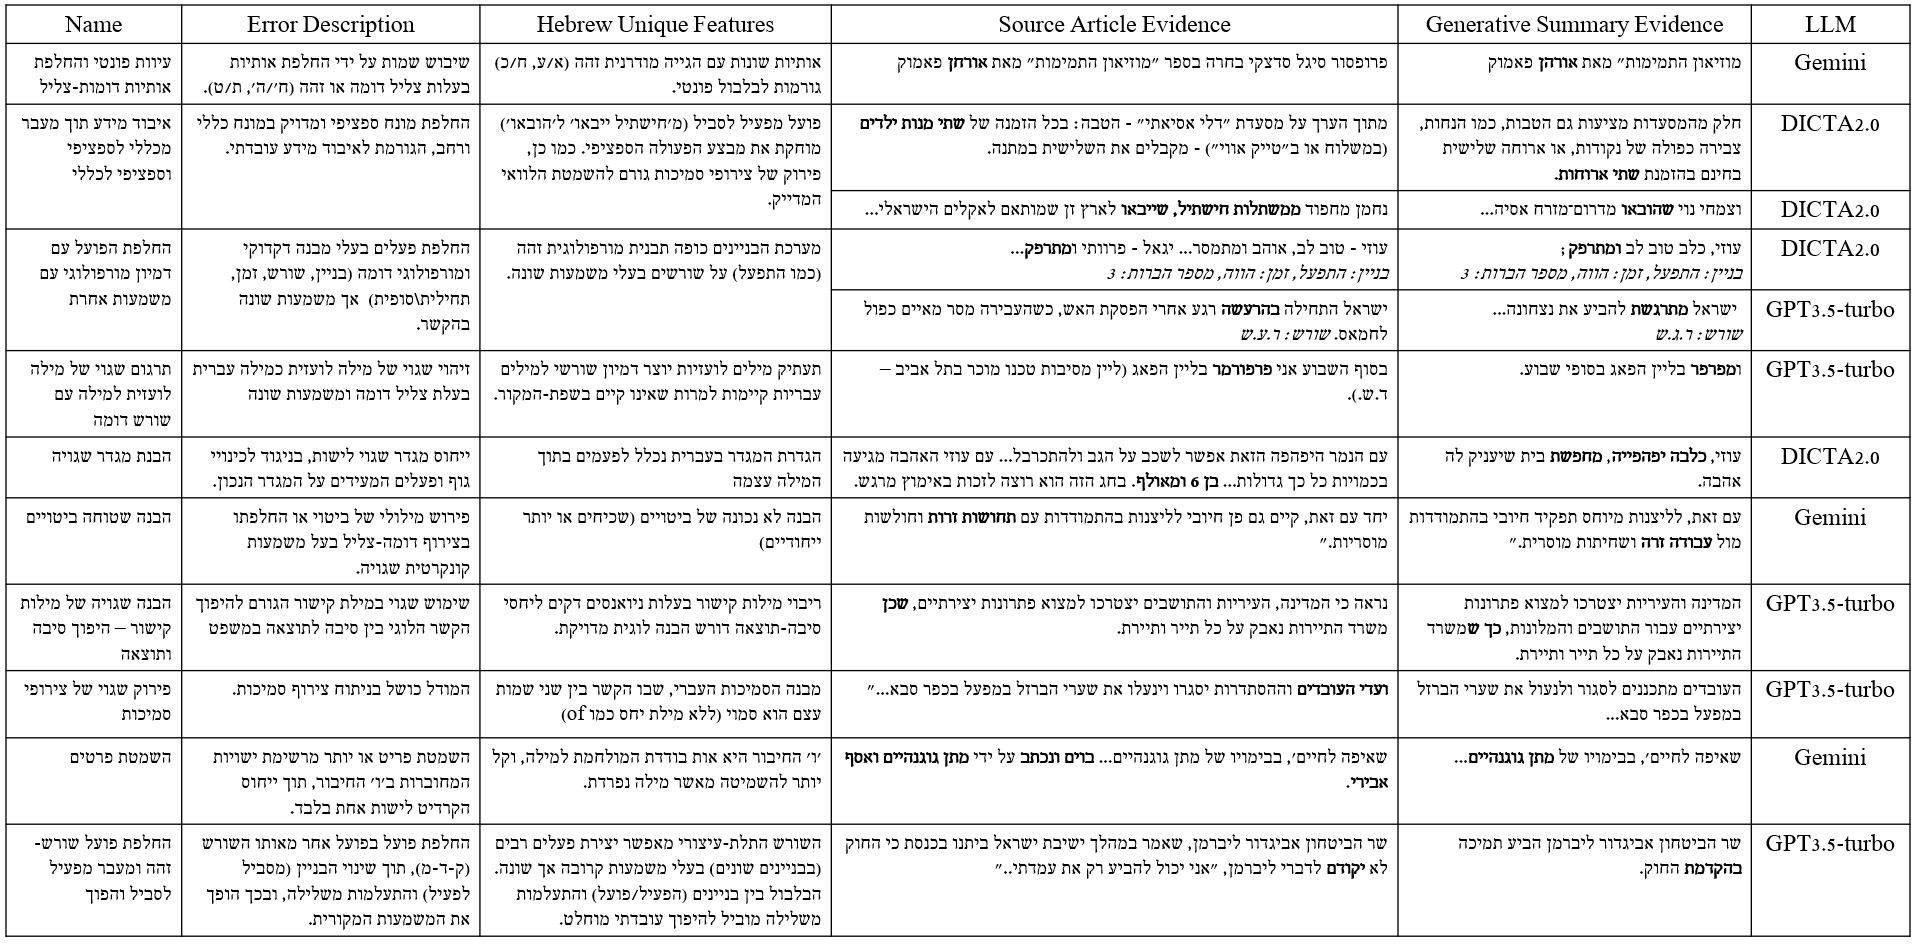
\includegraphics[width=\textwidth]{llm_error_analysis_hebrew.png}
\caption{Initial empirical analysis of factual errors in LLM-generated Hebrew summaries. Each row describes an error type, the Hebrew-specific features that give rise to it, evidence from the source article and the generated summary, and the LLM that produced it.}
\label{fig:llm_error_analysis}
\end{figure*}



\begin{figure*}[t]
\centering
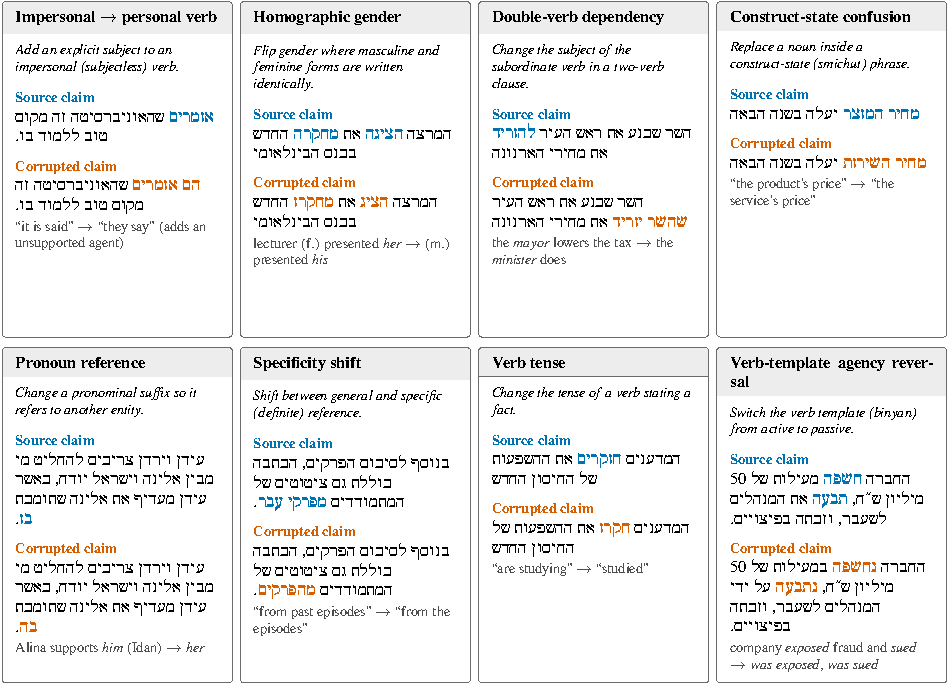
\includegraphics[width=\textwidth]{fig2_error_taxonomy_examples.pdf}
\caption{Eight of the 26 error families in the taxonomy. Each card gives the transformation rule, a faithful source claim (blue) and the corrupted claim (orange), with an English gloss of the change.}
\label{fig:taxonomy}
\end{figure*}

To ground the taxonomy in real model behavior, we generated about 300 summaries of MAFAT articles \citep{mafat_dataset} with DictaLM~2.0-Instruct, GPT-3.5-Turbo, and Gemini~1.5, used Claude~4 Sonnet and Gemini~2.5~Pro to flag factual inconsistencies with a severity score from 1 to 5, and had a native Hebrew speaker verify every error rated 4 or 5 (examples in Figure~\ref{fig:llm_error_analysis}). We derived the taxonomy from these verified errors. Classification followed a cross-linguistic transfer principle: an error was considered Hebrew-specific only if its underlying mechanism is intrinsically tied to the language's morpho-syntactic structure and occurs substantially more frequently in Hebrew than in morphologically simpler languages such as English.

Three criteria guided the taxonomy construction process: (1) \textbf{Morphological Dependency}, where the error arises from Hebrew's inflectional system (e.g., gender, number, binyan patterns, prefixes, and suffixes); (2) \textbf{Syntactic Uniqueness}, where the error involves Hebrew-specific constructions such as the construct state (\textit{smichut}); and (3) \textbf{Morphological Ambiguity}, where factual errors emerge from unclear word boundaries caused by affixation and morphological attachment.

Each candidate error type was independently evaluated by a Hebrew linguist against these criteria, with disagreements resolved through discussion. The resulting taxonomy (Figure~\ref{fig:taxonomy}) comprises 26 error families in three groups: (i) 17 Hebrew-specific morpho-syntactic families (e.g., \textit{verb\_gender\_swap}, \textit{construct\_state\_confusion}, \textit{hebrew\_root\_pattern\_confusion}, \textit{morphological\_connective\_confusion}); (ii) 3 cross-linguistic logical families (\textit{sentence\_negation}, \textit{number\_swap}, \textit{measure\_unit\_swap}); and (iii) 6 entity substitutions (person, location, organization, title, event, and date). Twenty families are operationalized in our augmentation pipeline (Section~\ref{sec:augmentation}); the remaining six morpho-syntactic families are defined but not yet used for generation. Each operationalized family is a blueprint for one controlled transformation of an otherwise faithful claim.

\section{Data Augmentation Pipeline}
Figure~\ref{fig:pipeline} gives an overview of the augmentation pipeline.

\begin{figure*}[t]
\centering
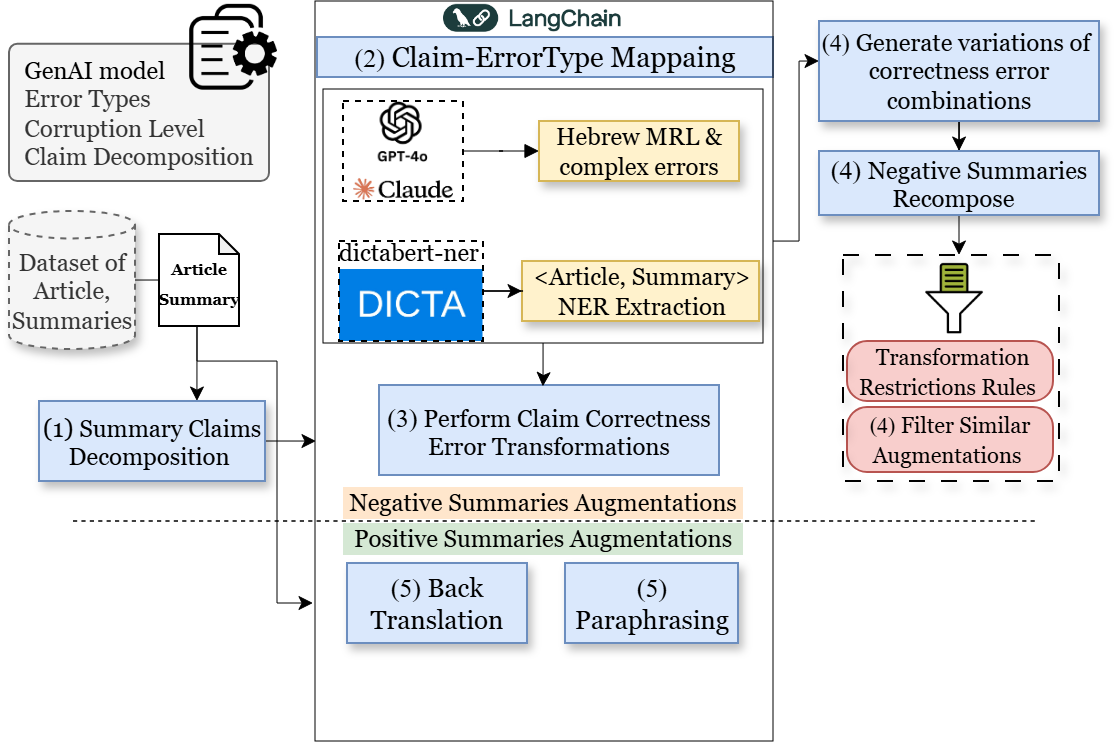
\includegraphics[width=0.8\textwidth]{dataset_creation.png}
\caption{Overview of the data augmentation pipeline: (1) summary claim decomposition; (2) claim--error-type mapping with LLMs and DictaBERT NER; (3) claim correctness error transformations; (4) generating error combinations, recomposing negative summaries, and filtering by transformation-restriction rules and similarity; (5) positive augmentations via back-translation and paraphrasing.}
\label{fig:pipeline}
\end{figure*}
\subsection{Source Documents}
We build on the MAFAT Hebrew summarization dataset \citep{mafat_dataset}, which pairs documents from five sources (Israel Hayom news, Wikipedia, the Weizmann Institute, the Knesset, and High Court of Justice rulings) with Hebrew reference summaries $S$. MAFAT references are either written by annotators (\emph{gold}) or drafted by an LLM and then reviewed, and in most cases edited, by an annotator (\emph{silver}).

\subsection{Augmentation and Labeling}
\label{sec:augmentation}

\paragraph{Negative summaries.}
Unlike prior injection pipelines, whose operators edit entities, numbers or negation, most of our operators act on Hebrew morphology, producing negatives that remain grammatical but contradict the source. Each reference summary is split into sentence-level claims $c_1,\dots,c_n$, and candidate edits are proposed by one of three mechanisms, depending on the family. (i) For the 11 Hebrew-specific families and four general families (negation, measure units, events, and dates), an LLM first marks the claims and spans to which each family applies and then rewrites each span with family-specific few-shot prompts. (ii) For person, location, organization, and title swaps, DictaBERT-NER \citep{shmidman2023dictabert} detects entities in the summary, and each is replaced by a different entity of the same type taken from the source article, so the substitution is plausible yet contradicts the source; candidates with normalized Levenshtein similarity of $0.57$ or more to the original are avoided. (iii) Numbers are changed by a deterministic rule (doubling). Edits that leave a claim unchanged are discarded. Span selection and rewriting use OpenAI GPT and Google Gemini models; in the final configuration, Gemini rewrites the root-pattern, idiom, connective, directional-preposition, and construct-state families and GPT the others.
% CHECK (audit B): git history shows gpt-4o + gemini-2.0-flash until 2025-11-16 and gpt-4.1 + gemini-2.5-pro after;
% all-OpenAI 2025-10-08..11-21, per-family Gemini mapping from 11-21. Name exact versions once confirmed.

Let $T$ be the total number of candidate edits for a summary. A negative summary combines
\begin{equation}
  m = \max\bigl(1, \lfloor \rho\, T \rfloor\bigr)
  \label{eq:num_errors}
\end{equation}
of these edits, where the corruption rate $\rho$ controls how heavily a summary is corrupted ($\rho=0.9$ in all experiments). We enumerate allocations of the $m$ edits to claims (at most $20{,}000$), applying at most one edit per family to a claim and never combining negation with another edit on the same claim, and substitute the edited claims back into the summary. Each negative inherits the set $E$ of families injected into it.

\paragraph{Diversity filter.}
To avoid near-duplicate negatives, we measure the surface overlap $o(a,b)$ between two summaries as the larger of their word-unigram and word-bigram Jaccard similarities. Among the first 51 recomposed candidates, a candidate $S'$ with error set $E'$ is kept only if $o(S',S)\le\theta(S')$ and $o(S',S'')\le\theta(S')$ for every candidate $S''$ already kept, with threshold
\begin{equation}
  \theta(S') = \theta_0 + 0.0013\,|E'|^{0.75},
  \label{eq:threshold}
\end{equation}
where $\theta_0=0.85$. The small allowance grows with the number of injected families, since each additional error is a further small edit to the same summary. At most seven negatives are kept per reference summary.
% CHECK (code): in utils.filter_diverse_summaries the threshold is updated
% cumulatively (max_same = max_same + ...) inside the loop, so it grows with
% every candidate examined, not per candidate as in Eq. (2). Fix the code to
% use a per-candidate threshold, or describe the actual behavior here.
% CHECK (code): if no candidate passes the filter, all candidates are kept
% unfiltered (then truncated to seven). Decide whether to report this fallback.

\paragraph{Positive summaries.}
Faithful positives are generated by an OpenAI GPT model prompted to rewrite a reference summary twice, once by back-translation through English and once by paraphrasing, while preserving every entity, number, negation, and causal connective as well as gender, tense, definiteness, and construct-state relations.

\paragraph{Labels.}
Within MAFAT-Aug, labels follow from construction: MAFAT reference summaries and their meaning-preserving rewrites are treated as faithful, and injected variants as unfaithful.

\section{MorphEvalHeb}
\label{sec:model}

\subsection{Binary Faithfulness Verifier}
\label{sec:binary}
The verifier is NeoDictaBERT fine-tuned as a sequence-pair classifier: the article and the summary are encoded together, truncated to 4,096 tokens, and a classification head predicts faithful or unfaithful. It is trained with cross-entropy. The MorphEvalHeb score of a summary is the predicted probability of the faithful class.
% Resolved: released checkpoint labels = ['contradiction', 'entailment'] (index 1 = faithful).

\subsection{Multi-label Error Detector}
\label{sec:multilabel}
The detector predicts which error families a summary contains. It uses the same encoder with one independent sigmoid output per family, and predicts every family whose probability is at least 0.5. Error families are highly imbalanced, so we train with binary cross-entropy in which each family's positive examples are weighted by that family's ratio of negative to positive training instances, and we oversample instances that contain rare families.

% CHECK (audit D): docs + HF card say Setup 2 premise = ORIGINAL claim (not the article); the released Setup 3
% was trained on (original claim, corrupted claim) with no evidence. Confirm, then fix this sentence and Figure 5.
We compare three input granularities (Figure~\ref{fig:setups}): the full article and summary (Setup~1, up to 4,096 tokens); the article and a single claim (Setup~2, up to 3,072 tokens); and a single claim with the top-$k$ evidence sentences retrieved from the article (Setup~3, up to 512 tokens).

\begin{figure*}[t]
\centering
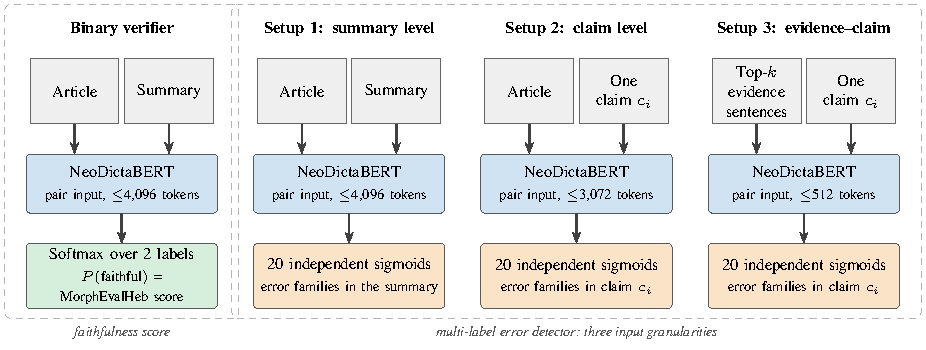
\includegraphics[width=\textwidth]{fig4_model_setups.pdf}
\caption{The MorphEvalHeb classifiers. All four fine-tune NeoDictaBERT on sequence pairs. The binary verifier outputs the probability that a summary is faithful, which serves as the MorphEvalHeb score; the multi-label detector predicts which of the 20 operationalized error families are present, at three input granularities.}
\label{fig:setups}
\end{figure*}

\section{Experimental Setup}
\subsection{Datasets}
\label{sec:datasets}
Our benchmark combines two sources that differ in how errors arise. \textbf{MAFAT-Aug} contains 1,889 article--summary pairs built from 303 MAFAT articles with the pipeline of Section~\ref{sec:augmentation}: 639 faithful summaries (209 MAFAT references, of which 77 are gold, 89 are LLM drafts edited by an annotator, and 43 are LLM drafts left unchanged; and 430 LLM back-translations or paraphrases of them) and 1,250 unfaithful summaries with injected errors. Its articles have a median length of 1,034 words and its reference summaries 142 words. \textbf{mFACT-He} adds 2,135 pairs (1,077 faithful, 1,058 unfaithful) with naturally occurring errors: mFACT \citep{qiu2023detecting} labels journalist-written XSum summaries as faithful or hallucinated by ranking them with an ensemble of four English faithfulness metrics, and we translated its test split from English into Hebrew with GPT-4o-mini. These summaries are much shorter (median 16 words), and their labels are automatic rather than human. Articles are assigned to training, validation, and test splits before augmentation, so all variants of an article fall into the same split. The binary verifier is trained on 18,238 pairs and evaluated on 2,239 validation and 2,918 test pairs; the claim-level Setup~3 detector uses 65,510, 17,004, and 41,650 claims, respectively.
% combined.csv = test_mfact.csv (2,135) + bk_combined.csv (430) + mafat_combined.csv (1,459); see benchmark/combination_summary.txt.
% CHECK: confirm combined.csv is disjoint from the binary verifier's 18,238 training pairs.
\subsection{Baseline Metrics}

We compare MorphEvalHeb against a comprehensive set of automatic evaluation metrics spanning five major paradigms.

\paragraph{N-gram and Surface Metrics.}
We evaluate \textbf{ROUGE-1}, \textbf{ROUGE-2}, and \textbf{ROUGE-L} \cite{lin2004rouge}, which measure unigram, bigram, and longest common subsequence overlap between the summary and the source document. We additionally compute \textbf{BLEU} \cite{papineni2002bleu}, \textbf{ChrF} \cite{popovic2015chrf}, and \textbf{Token F1} following the formulation of \citet{honovich2022true}. To quantify abstractiveness, we report the percentage of novel unigrams, bigrams, and trigrams not appearing in the source document \citep{aharoni-etal-2023-multilingual}.

\paragraph{Semantic Similarity.}
We evaluate \textbf{BERTScore} \cite{zhang2020bertscore}, which measures semantic similarity using contextual embeddings. To assess the effect of encoder choice, we report results using three Hebrew language models: \texttt{avichr/heBERT}, \texttt{onlplab/alephbert-base} \citep{seker-etal-2022-alephbert}, and \texttt{dicta-il/neodictabert} \citep{shmidman2023dictabert}.

\paragraph{NLI-Based Factuality.}
We implement \textbf{SummaC-ZS} \cite{DBLP:journals/corr/abs-2111-09525}, replacing the original English-only NLI backbone with the multilingual model \texttt{MoritzLaurer/mDeBERTa-v3-base-mnli-xnli} \cite{laurer-etal-2022-deberta}. Consistency scores are computed using sentence-level entailment aggregation as proposed by the original framework.

% TODO (QAFactEval, required before submission): not yet scored on the benchmark -- the author will give
%   instructions. Run summary_augmentation/pages/metrics/qa_facteval.py PipelineFactory.hybrid(client,
%   openai_model="gpt-4o-mini") on all 4,024 pairs (factory default is gpt-3.5-turbo -- pass the model
%   explicitly). Needs: OPENAI_API_KEY (rotated), dicta-il/dictabert-syntax, deepset/xlm-roberta-large-squad2.
%   Est. ~55k questions, ~$3-5 (hybrid) / ~$15-25 (fully generative). Then fill its row in Table 1
%   (tab:main_results) and Table 4 (tab:full_results).
\paragraph{QA-Based Factuality.}
We implement a Hebrew adaptation of \textbf{QAFactEval} \cite{fabbri-etal-2022-qafacteval}. Since the original pipeline relies on English-only components, we evaluate two Hebrew-capable configurations. The \emph{hybrid} configuration combines DictaBERT dependency parsing \cite{shmidman2023dictabert}, \texttt{GPT-4o-mini} question generation, and \texttt{deepset/xlm-roberta-large-squad2} extractive question answering. The \emph{fully generative} configuration uses \texttt{GPT-4o-mini} for question generation, answer extraction, and answer comparison. Final scores are computed by averaging answer-level consistency scores across generated questions.

\paragraph{LLM-as-Judge Metrics.}
We evaluate \textbf{G-EVAL} \cite{liu-etal-2023-g}, which uses chain-of-thought prompting to score factuality, and a \textbf{vanilla zero-shot LLM judge} that directly assesses factual consistency without structured evaluation criteria. Both methods employ \texttt{GPT-4o-mini} with deterministic decoding.

\paragraph{Entity Hallucination.}
\textbf{ENFS} \citep{cao-etal-2022-hallucinated} is the share of named entities in the summary, detected with DictaBERT-NER \citep{shmidman2023dictabert}, that do not appear among the source's entities; we negate it so that higher means more faithful.

\paragraph{Trained Fact Checker.}
\textbf{FactCG} \citep{lei-etal-2025-factcg} is a DeBERTa-v3-large fact checker trained on graph-based multi-hop synthetic data, among the strongest small checkers on English grounding benchmarks. We apply the released English model to Hebrew as a cross-lingual baseline, following its reference inference: the source is split into sentence-aligned chunks of up to 550 tokens, and the score is the probability that the summary is supported, maximized over chunks.

\paragraph{Trained Hebrew Classifier.}
\textbf{mFACT-He} follows the mFACT recipe \citep{qiu2023detecting}: NeoDictaBERT, the same encoder as ours, fine-tuned only on the Hebrew translation of the mFACT training data. It therefore isolates the effect of our training data. MorphEvalHeb's binary verifier is trained on the training splits of both MAFAT-Aug and mFACT-He.

\paragraph{Generation Probability Metrics.}
We evaluate \textbf{BARTScore} \cite{yuan2021bartscore}, which measures the conditional likelihood of a summary given its source document under a pre-trained sequence-to-sequence model; we use \texttt{facebook/bart-large-cnn}, an English model, so BARTScore serves only as a reference point for Hebrew.




\subsection{Evaluation Protocol}
\label{sec:protocol}
We compare each metric's scores with the binary faithfulness labels of the test summaries using three statistics. \textbf{Kendall's $\tau_b$}: because the labels are binary, most pairs of summaries are tied in the label, so we use the tie-adjusted $\tau_b$ variant \citep{deutsch-etal-2023-ties}. \textbf{ROC AUC}, which needs no decision threshold and is unaffected by the label imbalance, following the recommendation of \citet{honovich2022true}. \textbf{Balanced accuracy}, the mean of the true-positive and true-negative rates; for every metric we choose the decision threshold the same way, maximizing balanced accuracy on four of five article-grouped folds and applying it to the fifth, so no threshold is tuned on the data it is scored on. We report balanced accuracy rather than plain accuracy because the benchmark is imbalanced: a majority-class baseline already reaches 57.4\% accuracy overall and 66.2\% on MAFAT-Aug alone (Table~\ref{tab:full_results}), while its balanced accuracy is 0.5 by construction on every part.

\paragraph{Uncertainty and significance.}
Following \citet{deutsch-etal-2021-statistical}, we report 95\% confidence intervals from a percentile bootstrap that resamples articles, keeping all summaries of an article together ($B=1000$ resamples). To test whether metric $A$ outperforms metric $B$, we use a paired bootstrap: both metrics are evaluated on the same resampled instances, and the one-sided $p$-value is the fraction of resamples in which $A$'s AUC is not higher than $B$'s. We correct for multiple comparisons against MorphEvalHeb with the Holm--Bonferroni procedure.
% Implemented in paper/results/eval/analyze.py (scores: run_eval.py -> scores.csv).

\subsection{Implementation Details}
All classifiers fine-tune \texttt{dicta-il/neodictabert} \citep{BenDavid2025neodictabert} (363M parameters) with a learning rate of $2\times10^{-5}$ and AdamW. The binary verifier is trained for one epoch with an effective batch size of 16, keeping the checkpoint with the best validation F1. The multi-label detectors use an effective batch size of 32, a cosine schedule, and two epochs (Setups~1 and~2) or one epoch (Setup~3). Training used a single NVIDIA RTX~6000 Ada GPU; the binary verifier trained in about three hours.

\section{Results}

\subsection{Meta-Evaluation}
\label{sec:meta_eval}
\begin{table}[t]
\centering
\small
\setlength{\tabcolsep}{3pt}
\renewcommand{\arraystretch}{1.35}
\begin{tabular}{lcc}
\toprule
\textbf{Metric} & \textbf{Kendall $\tau$} & \textbf{Kendall $\tau_b$} \\
 & \textit{original run} & \textit{[95\% CI]} \\
\midrule
\textbf{MorphEvalHeb} (ours) & \textbf{0.6996} & \shortstack{\textbf{0.689}\\{\scriptsize[0.68,0.70]}} \\
\midrule
Vanilla Model (zero-shot judge) & 0.5989 & pending \\
mFACT & 0.5290 & pending \\
G-EVAL & 0.2418 & pending \\
ENFS & -- & \shortstack{0.265\\{\scriptsize[0.23,0.30]}} \\
ROUGE-2 & -- & \shortstack{0.009\\{\scriptsize[-0.02,0.05]}} \\
BERTScore (AlephBERT) & -- & \shortstack{-0.013\\{\scriptsize[-0.04,0.02]}} \\
SummaC & 0.0064 & \shortstack{0.125\\{\scriptsize[0.10,0.16]}} \\
QAFactEval (hybrid) & -- & pending \\
FactCG & -- & pending \\
BERTScore (heBERT) & 0.0162 & \shortstack{-0.061\\{\scriptsize[-0.09,-0.03]}} \\
Token F1 & -- & \shortstack{-0.071\\{\scriptsize[-0.10,-0.04]}} \\
ROUGE-1 & 0.1391 & \shortstack{-0.093\\{\scriptsize[-0.12,-0.06]}} \\
ROUGE-L & -- & \shortstack{-0.094\\{\scriptsize[-0.12,-0.06]}} \\
BLEU & -- & \shortstack{-0.105\\{\scriptsize[-0.14,-0.07]}} \\
chrF & -- & \shortstack{-0.209\\{\scriptsize[-0.23,-0.18]}} \\
\bottomrule
\end{tabular}
\renewcommand{\arraystretch}{1}
\caption{Kendall's $\tau$ between metric scores and the reference faithfulness labels on the Hebrew benchmark ($n{=}4{,}024$). Higher values indicate stronger agreement with the labels. Bold marks our method. The first column reports our original run; the second re-computes the tie-adjusted $\tau_b$ with the protocol of Section~\ref{sec:protocol}, with 95\% bootstrap confidence intervals over articles (``pending'': not yet re-run). Appendix~\ref{app:full_results} gives AUC and balanced accuracy for each benchmark part.}
\label{tab:main_results}
\end{table}


Table~\ref{tab:main_results} compares Kendall's $\tau$ across all metrics; Table~\ref{tab:full_results} (Appendix~\ref{app:full_results}) adds AUC and balanced accuracy for each benchmark part.
% CHECK: these labels come from construction (Section~4.2), not from human annotators.
% If a human-annotated subset exists, report it separately.



MorphEvalHeb reaches an AUC of 0.992 (95\% CI 0.987--0.996), a balanced accuracy of 0.969, and $\tau_b$ of 0.689, and it is equally strong on injected errors (MAFAT-Aug) and on naturally occurring errors in journalist-written summaries (mFACT-He), with an AUC of 0.995 on each. Surface-overlap and embedding metrics are near chance on MAFAT-Aug (AUC 0.50--0.55), since an injected morphological error leaves almost every token in place; several fall below 0.5 overall because faithful rewrites change more tokens than corruptions do. Among the recomputed baselines, ENFS is the strongest (AUC 0.677), mainly on mFACT-He, whose naturally occurring errors often introduce new entities (see Appendix~\ref{app:enfs} for its Hebrew-specific failure mode); among the LLM judges evaluated so far, the zero-shot GPT-4o-mini judge is the strongest ($\tau=0.599$), despite MorphEvalHeb's 363M-parameter encoder being far smaller than the LLM judges it outperforms.

\subsection{Binary Faithfulness Verification}
\label{sec:res_binary}
On its own held-out test split (2,918 pairs), the verifier reaches 96.6\% accuracy, balanced accuracy 96.7\% (95\% CI 96.1--97.3), AUC 0.990 (0.987--0.993), and $\tau_b$ 0.684, consistent with Table~\ref{tab:main_results}.
% CHECK: Table 1 (combined.csv) and this test split share only 8 pairs. Confirm that combined.csv
% was excluded from the verifier's 18,238 training pairs, otherwise Table 1 is optimistic.
% TODO: score the baselines on this same test split so both evaluations line up.

\paragraph{Calibration and selective prediction.} Beyond discrimination, MorphEvalHeb's probability is well-calibrated on the full benchmark ($n{=}4{,}024$): Brier score 0.0281 (0.25 for an uninformative constant-0.5 predictor) and expected calibration error 0.0256 (10 bins), so the score is usable as a continuous risk estimate rather than only a binary decision. It also supports selective prediction: abstaining only on the pairs within $\pm0.1$ of the decision threshold flags just 10 pairs (0.25\%) for human review, and that small flagged set concentrates the hard cases, with 30\% accuracy on the flagged pairs versus 96.9\% overall.

\subsection{Multi-label Error Detection}
\label{sec:res_multilabel}
The released Setup~3 checkpoint, trained and tested on pairs of a summary claim and its original claim, reaches a micro-averaged F1 of 0.787 (precision 0.674, recall 0.945) on 41,650 test pairs; since it sees the uncorrupted claim, this measures error typing rather than reference-free detection.
% TODO (required): Setup 1 and Setup 2 test results (not in the released model repos), and
%   per-family F1 for Setup 3 -- the released predictions.csv has an empty ground-truth column,
%   so per-family scores need the server's test.csv.

\subsection{Analysis}
\label{sec:analysis}
\paragraph{Difficulty.} Using each metric's MAFAT-Aug decision threshold, MorphEvalHeb flags 93\% of negatives with a single injected error family ($n{=}45$) and 90--99\% at every number of families, whereas the best surface or embedding baseline flags at most 43\% at any level.

\paragraph{Robustness to meaning-preserving rewrites.} Following \citet{mujahid-etal-2026-stress}, we compare scores of 208 reference summaries with their faithful rewrites: MorphEvalHeb's score moves by under 0.01 standard deviations, while ROUGE-2 drops by 0.32 and BERTScore by 0.10. The verifier saw such rewrites in training, so this is partly in-distribution.

\section{Conclusion}
We presented MorphEvalHeb, a Hebrew-native factual-consistency framework built on a taxonomy of 26 error families derived from real LLM summaries and a morphology-aware augmentation pipeline. MorphEvalHeb separates faithful from unfaithful Hebrew summaries with an AUC of 0.992, while surface and embedding metrics stay near chance. Future work will add human judgments of native LLM summaries, the remaining six error families, and other generation tasks, including the intermediate summarization steps inside Hebrew-speaking LLM agent pipelines, where an unfaithful summary can propagate into downstream actions.

\section*{Limitations}
\textbf{No human faithfulness labels.} Neither part of the benchmark is labeled by human annotators: MAFAT-Aug labels follow from construction, so references are assumed faithful even though 132 of its 209 references are LLM drafts (43 left unedited) that may contain errors, and its injected errors need not match those of real summarizers \citep{goyal-durrett-2021-annotating}; mFACT-He contains naturally occurring errors, but its labels come from English metrics and its texts are machine-translated. Human faithfulness judgments of native Hebrew summaries produced by current LLMs are needed to confirm our findings.

\textbf{Error coverage and difficulty.} Only 20 of the 26 taxonomy families are used for generation, and a negative summary combines a median of seven families; detection stays high for single-error negatives (Section~\ref{sec:analysis}), but only 45 such negatives exist, so single subtle errors remain under-tested.

\textbf{Dependence on proprietary LLMs.} Span selection, error rewriting, and positive rewriting rely on Gemini and GPT models whose behavior can change across versions, and the pipeline does not automatically verify that edited claims remain grammatical.

\textbf{Data and scope.} The MAFAT part of the benchmark covers 303 articles from five sources; more than half of the benchmark is mFACT data translated by an LLM, which has much shorter summaries and shares its origin with the mFACT baseline. The error statistics in Figure~\ref{fig:llm_detected_errors} are produced automatically. We study summarization only, with a single LLM-judge model (GPT-4o-mini).

\section*{Ethics Statement}
All source documents are drawn from the public MAFAT Hebrew summarization dataset \citep{mafat_dataset} (news, Wikipedia, Weizmann Institute, Knesset, and High Court of Justice text) and from the mFACT Hebrew translations \citep{qiu2023detecting}; neither contains personal or sensitive information beyond what is already public. No new human-subject data collection was performed: the taxonomy was validated by a Hebrew linguist and a native Hebrew speaker, as described in Section~\ref{sec:taxonomy}, and the benchmark labels follow automatically from the augmentation pipeline (Section~\ref{sec:augmentation}) rather than from crowdsourced annotation. Data generation and the baseline LLM judges rely on commercial LLM APIs (OpenAI GPT and Google Gemini models); we use them only to rewrite or score Hebrew text already present in the source datasets, not to generate content about individuals.

\bibliography{custom}

\appendix

\section{Full Meta-Evaluation Results}
\label{app:full_results}
\begin{table*}[t]
\centering
\small
\setlength{\tabcolsep}{5pt}
\begin{tabular}{lccc|cc|cc}
\toprule
 & \multicolumn{3}{c|}{\textbf{All} ($n{=}4{,}024$)} & \multicolumn{2}{c|}{\textbf{MAFAT-Aug} ($n{=}1{,}889$)} & \multicolumn{2}{c}{\textbf{mFACT-He} ($n{=}2{,}135$)} \\
\textbf{Metric} & AUC [95\% CI] & BAcc & $\tau_b$ & AUC & BAcc & AUC & BAcc \\
\midrule
\multicolumn{8}{l}{\textit{Trivial baseline}} \\
Majority class & 0.500 & 0.500 & -- & 0.500 & 0.500 & 0.500 & 0.500 \\
\multicolumn{8}{l}{\textit{Surface overlap}} \\
ROUGE-1 & 0.434\,{\scriptsize[0.41,0.46]} & 0.522 & -0.093 & 0.508 & 0.505 & 0.527 & 0.562 \\
ROUGE-2 & 0.506\,{\scriptsize[0.48,0.53]} & 0.579 & 0.009 & 0.514 & 0.532 & 0.696 & 0.713 \\
ROUGE-L & 0.433\,{\scriptsize[0.41,0.46]} & 0.517 & -0.094 & 0.505 & 0.530 & 0.504 & 0.547 \\
BLEU & 0.447\,{\scriptsize[0.43,0.47]} & 0.499 & -0.105 & 0.495 & 0.499 & 0.501 & 0.497 \\
chrF & 0.350\,{\scriptsize[0.33,0.37]} & 0.497 & -0.209 & 0.515 & 0.500 & 0.301 & 0.504 \\
Token F1 & 0.449\,{\scriptsize[0.43,0.47]} & 0.525 & -0.071 & 0.502 & 0.514 & 0.571 & 0.585 \\
\multicolumn{8}{l}{\textit{Embedding similarity}} \\
BERTScore (heBERT) & 0.456\,{\scriptsize[0.44,0.48]} & 0.533 & -0.061 & 0.517 & 0.513 & 0.598 & 0.599 \\
BERTScore (AlephBERT) & 0.491\,{\scriptsize[0.47,0.52]} & 0.551 & -0.013 & 0.547 & 0.541 & 0.678 & 0.631 \\
\multicolumn{8}{l}{\textit{Entity hallucination}} \\
ENFS (entity overlap) & 0.677\,{\scriptsize[0.65,0.70]} & 0.639 & 0.265 & 0.652 & 0.605 & 0.739 & 0.745 \\
\multicolumn{8}{l}{\textit{NLI}} \\
SummaC-ZS (mDeBERTa) & 0.589\,{\scriptsize[0.57,0.61]} & 0.573 & 0.125 & 0.645 & 0.593 & 0.710 & 0.642 \\
\multicolumn{8}{l}{\textit{Trained classifier}} \\
mFACT-He$^{\ddagger}$ & -- & -- & 0.529 & -- & -- & -- & -- \\
\multicolumn{8}{l}{\textit{Trained fact checker (cross-lingual)}} \\
FactCG & -- & -- & pending & -- & -- & -- & -- \\
\multicolumn{8}{l}{\textit{LLM judge (GPT-4o-mini)}} \\
Zero-shot judge$^{\ddagger}$ & -- & -- & 0.599 & -- & -- & -- & -- \\
G-EVAL$^{\ddagger}$ & -- & -- & 0.242 & -- & -- & -- & -- \\
\midrule
\textbf{MorphEvalHeb} (ours) & \textbf{0.992\,{\scriptsize[0.99,1.00]}} & \textbf{0.969} & \textbf{0.689} & \textbf{0.995} & \textbf{0.980} & \textbf{0.995} & \textbf{0.968} \\
\bottomrule
\end{tabular}
\caption{Full meta-evaluation on the Hebrew benchmark. Bold marks our method. AUC and Kendall's $\tau_b$ are threshold-free; balanced accuracy (BAcc) uses a decision threshold tuned on held-out folds (Section~\ref{sec:protocol}). Brackets give 95\% bootstrap confidence intervals over articles. MorphEvalHeb outperforms every recomputed baseline ($p<0.001$, paired bootstrap on AUC, Holm-corrected). $^{\ddagger}$Not yet recomputed: $\tau$ from our earlier run; the remaining columns are pending.}
\label{tab:full_results}
\end{table*}




\section{Hebrew Morphology and Entity Matching}
\label{app:enfs}
Named entities themselves fragment less under the NeoDictaBERT tokenizer than the Hebrew tokens around them (1.00 vs.\ 1.24 subword tokens per word on average, $n{=}2{,}875$ documents, Wilcoxon $p<0.001$), so ENFS's failures do not come from entities being heavily subworded. ENFS flags at least one unsupported entity in 86\% of faithful MAFAT-Aug summaries. Stripping Hebrew proclitic prefixes before matching lowers this to 74\% but does not improve discrimination (AUC 0.660), so prefix handling alone does not make entity overlap a reliable Hebrew metric.

\end{document}
